\documentclass[10pt,twoside,draft]{book}
\usepackage{../../thesis}
\graphicspath{ {../../images/} }
\usetikzlibrary{arrows,positioning} 
\tikzset{
    %Define standard arrow tip
    >=stealth',
    %Define style for boxes
    box/.style={
           rectangle,
           rounded corners,
           draw=black, very thick,
           text width=6.5em,
           minimum height=2em,
           text centered},
    % Define arrow style
    imply/.style={
           ->,
           thick,
           shorten <=2pt,
           shorten >=2pt},
    both/.style={
           <->,
           thick,
           shorten <=2pt,
           shorten >=2pt,},
    induced/.style={
           dotted,
           ->,
           thick,
           shorten <=2pt,
           shorten >=2pt},
    maybe/.style={
           ->, 
           -o,
           thick,
           shorten <=2pt,
           shorten >=50pt},
    noimply/.style={
           ->, %inden[
         -],
           thick,
           shorten <=2pt,
           shorten >=60pt}
}


\makeindex

\begin{document}
\label{chap:comparison}
\chapter{Comparisons of Definitions of Chaos}
We have seen four definitions 
\begin{enumerate}[(i)]
  \item Devaney (\dev)
  \item Li-Yorke (\liy)
  \item Block-Coppel (\blcp)
  \item Positive topological entropy (\pte)
\end{enumerate}
and their variants
\begin{itemize}
  \item Wiggins's (similar to Devaney) (\wig)
  \item Martelli (equivalent to Wiggins's in $\R^n$)
  \item Marotto (implies Li-Yorke. Requires differentiability)
\end{itemize}
In this chapter, we discuss the relations between the definitions (i)$\sim$(iv) and Wiggins's definition.
Throughout this chapter, we consider the dynamical system $(X,F)$, where $X$ is a compact metric space, and $F$ is a continuous mapping.
We first discuss a special case when $X$ is a compact interval, then proceed to the general case.
%%%

\section{Compact Interval}
Let $I \subseteq \R$ be a compact interval.
In this section, we consider the case when $X = I$.
We show that Devaney's, Block-Coppel's, and positive topological entropy are equivalent conditions, and any of the three implies Li-Yorke's chaos.
\begin{figure}[ht]
  \centering
  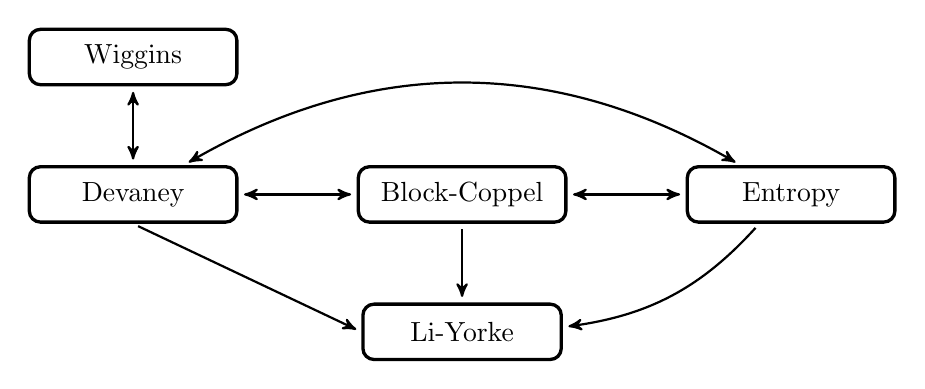
\begin{tikzpicture}[node distance=1cm, auto,]
 %nodes
    \node[box] (ly) {Li-Yorke};
    \node[box, inner sep=5pt,above=1.0cm of ly] (bc) {Block-Coppel};
    \node[box, inner sep=5pt,left=1.5cm of bc] (dev) {Devaney};
    \node[box, inner sep=5pt,right=1.5cm of bc] (ent) {Entropy};
    \node[box, inner sep=5pt,above=1.0cm of dev] (wig) {Wiggins};
 %edges
    \draw[imply] (dev.south) to node[bend right=20] {} (ly.west);  %this guy doesn't bend
    \draw[imply] (ent) to[bend left=20] node {} (ly); 
    \draw[imply] (bc) to node {} (ly); 
    \draw[both] (dev) to[bend left=30] node {} (ent); 
    \draw[both] (dev) to node {} (bc); 
    \draw[both] (dev) to node {} (wig); 
    \draw[both] (bc) to node {} (ent); 
  \end{tikzpicture}
  \label{fig:chaos-interval}
  \caption{
    Relations between the four definitions for the compact interval case.
    The three definitions in the top row are all equivalent.
    Li-Yorke's definition is strictly weaker than the other three.
  }
\end{figure}

\subsubsection*{Devaney/Wiggins and Block-Coppel}
We already mentioned in Chapter~\ref{chap:devaney} that \dpp and \tt imply \sdic in a compact metric space.
Moreover, on a compact interval, topological transitivity implies the existence of dense periodic points.
Thus, Devaney's and Wiggins's definitions are equivalent.
\begin{theorem}
  $(I,F)$ is chaotic in the sense of Devaney if and only if it is chaotic in the sense of Wiggins.
  \label{thm:devaney-wiggins}
  \begin{proof}
    It follows from the fact that \tt implies \dpp on a compact interval.
    See \citet{silverman} for the proof.
  \end{proof}
\end{theorem}
Also, \dev and \blcp are equivalent.
\begin{theorem}
  $(I,F)$ is chaotic in Devaney's sense if and only if it is chaotic in Block-Coppel's sense.
  \begin{proof}
    See \citet{aulbach}.
    %The proof uses \citep[VI: Proposition 6]{blockcoppel} .
  \end{proof}
  \label{thm:devaney-blockcoppel}
\end{theorem}
%%%

\subsubsection*{Block-Coppel and Positive Topological Entropy}
Block-Coppel's definition is equivalent to a mapping having positive topological entropy.
\begin{theorem}
  $(I,F)$ is chaotic in the sense of Block-Coppel if and only if $F: I \to I$ has positive topological entropy.
  \label{thm:entropy-blockcoppel}
  \begin{proof}
    See \citet[VII, Theorem 24]{blockcoppel}.
  \end{proof}
\end{theorem}
Hence, the three definitions---Devaney, Block-Coppel, and positive topological entropy---are equivalent.
%%%

\subsubsection*{Block-Coppel and Li-Yorke}
Next, we show that Block-Coppel's definition implies Li-Yorke's definition.
\begin{theorem}
  \citep{blockcoppel}
  If $(I,F)$ is chaotic in Block-Coppel's sense, then it is chaotic in Li-Yorke's sense.
  \label{thm:devaney-liyorke}
  \begin{proof}
    See \citet{blockcoppel} (VI; Proposition 27).
  \end{proof}
\end{theorem}
However, the coverse of the previous theorem is not true in general.
The following is an example of a dynamical system that is \liy but not \blcp.
\begin{example}
  (Truncated tent map \citep{aulbach})
  The tent map is defined as
  \begin{equation*}
    T(x) = 
    \begin{cases}
      2x     &\mbox{ if } x \in [0,1/2] \\
      2 - 2x &\mbox{ if } x \in [1/2,1].
    \end{cases}
  \end{equation*}
  We define the \textit{truncated tent map} for $\lambda \in [0,1]$ as 
  \begin{equation*}
    T_\lambda(x) = \min\set{\lambda, T(x)}.
  \end{equation*}
  (Thus, a truncated tent map is the tent map truncated at the height $\lambda$.
  Also, $T_1 = T$.)

  \begin{figure}[th]
    \centering
    \begin{tikzpicture}[scale=3.2]
      \draw[->] (-0.2,0) -- (1.2,0) node[right] {$x$};
      \draw[->] (0,-0.2) -- (0,1.2) node[above] {$T(x)$};
      \foreach \x/\xtext in {0.5/\frac{1}{2}, 1/1}
      \draw[shift={(\x,0)}] (0pt,1pt) -- (0pt,-1pt) node[below] {$\xtext$};
      \foreach \y/\ytext in {0.5/\frac{1}{2}, 0.8/\frac{4}{5}, 1/1}
      \draw[shift={(0,\y)}] (1pt,0pt) -- (-1pt,0pt) node[left] {$\ytext$};

      \draw[domain=0:0.4] plot (\x,{2*\x}) node[below right] {};
      \draw[domain=0.4:0.5, dotted] plot (\x,{2*\x}) node[below right] {};
      \draw[domain=0.5:0.6, dotted] plot (\x,{2 - 2*\x}) node[below right] {};
      \draw[domain=0.6:1] plot (\x,{2 - 2*\x}) node[below right] {};
      \draw[domain=0.4:0.6] plot (\x,{0.80}) node[below right] {};
    \end{tikzpicture}
    \label{fig:tent-map}
    \caption{The truncated tent map, $T_\lambda(x)$, for $\lambda = 4/5$.}
  \end{figure}
  Define a partition of $[0,1]$ by two sets
  \begin{equation*}
    J_\lambda \ceq \brac{0, \frac{\lambda}{2}} \cup \brac{1 - \frac{\lambda}{2}, 1} 
    \quad\mbox{ and }\quad
    K_\lambda \ceq \paren{\frac{\lambda}{2}, 1- \frac{\lambda}{2}}.
  \end{equation*}
  For any $0 \leq \lambda \leq \gamma \leq 1$, $T_\lambda$ and $T_\gamma$ coincide on $J_\lambda$.
  Furthermore, a point in $J_\lambda$ is a periodic point of $T_\gamma$ if and only if it is a periodic point of $T_\lambda$.

  The (untruncated) tent map $T_1$ has a 3-periodic point (e.g. $\set{2/7, 4/7, 6/7}$), so by Sarkovskii's theorem, $T_1$ has $2^n$-periodic points for all $n \in \N$.
  For any $n \in \N$, define
  \begin{equation*}
    \lambda_n \ceq \min\setst{\lambda \in [0,1]}{\mbox{ a } 2^n\mbox{-periodic orbit is contained in } [0,\lambda]}.
  \end{equation*}
  $\lambda_n$ exists for each $n$ because, for each $m \in \N$, the number of $m$-periodic points of $T_1$ is finite.
  To see this, note that $T_1$ has at most 2 fixed points, $\itr{T_1}{2}$ has at most $2^2$, and so on. 
  We can inductively show that the number of fixed points for $\itr{T_1}{m}$ is less than or equal to $2^m$. (Diagram)
  Also note that $\lambda_n$ is a $2^n$-periodic point of $T_1$ by construction.

  Next, we show that 
  \begin{equation*}
    O_{T_1}(\lambda_n) \subseteq J_{\lambda_n}.
  \end{equation*}
We have $T_1(K_{\lambda_n}) = (\lambda_n, 1]$, but by definition of $\lambda_n$, $O_{T_1}(\lambda_n)$ is contained in $[0,\lambda_n]$.
It follows that no point of $O_{T_1}(\lambda_n)$ is in $K_{\lambda_n}$, which implies $O_{T_1}(\lambda_n) \subseteq J_{\lambda_n}$.
Since $T_1$ and $T_{\lambda_n}$ coincide on $J_{\lambda_n}$, $\lambda_n$ is also a $2^n$-periodic point of $T_{\lambda_n}$, and its orbit under iteration by $T_{\lambda_n}$ is also contained in $J_{\lambda_n}$.
Then, by Sarkovskii's theorem, $T_{\lambda_n}$ has a periodic points of periods
\begin{equation*}
  2^n, 2^{n-1}, \ldots, 2, 1.
\end{equation*}
Furthermore, we show that no periodic point of $T_{\lambda_n}$ has a period different from these.
%We first prove that there cannot be more than one periodic point in $\cl(K_{\lambda_n})$ by contradiction. %%% Unnecessary?
%Suppose there exist $a,b \in \cl(K_{\lambda_n})$ that are periodic points of $T_{\lambda_n}$.
%Since $T_{\lambda_n}(a) = T_{\lambda_n}(b) = \lambda_n$, $a$ and $b$ are in the orbit of $\lambda_n$, so that the periods of $a$ and $b$ are $2^n$.
%We may suppose that $\itr{T}{k}(a) = b$ for some $0 < k < 2^n$ without loss of generality.
%Then,
%\begin{equation*}
%  \itr{T}{k}(a) = b 
%  \Rar 
%  \itr{T}{k+1}(a) = T(b)
%  \Rar 
%  \itr{T}{k}(\lambda_n) = \lambda_n,
%\end{equation*}
%which implies that $\lambda_n$ has period less than $2^n$, a contradiction.
To prove claim, suppose on the contrary that $T_{\lambda_n}$ has a $m$-periodic point $p$, where $m$ is an integer that comes before $2^n$ in the Sarkovskii's ordering.
Denote $O_{T_{\lambda_n}}(p)$, the orbit of $p$, by $M$.
Since $T_{\lambda_n}$ can only have periodic points of period $2^n$ in $K_{\lambda_n}$, no point in $M$ is contained in $K_{\lambda_n}$, which means that
\begin{equation*}
  M \subseteq J_{\lambda_n}.
\end{equation*}
Now, define $\rho \ceq \max M$.
Since the period of $\rho$ is not $2^n$, it cannot be $\lambda_n$.
It follows that
\begin{equation*}
  \rho < \lambda_n.
\end{equation*}
Then, by Sarkovskii's theorem, there exists a $2^n$-periodic point in $[0,\rho] \subsetneq [0, \lambda_n]$.
This contradicts the fact that $\lambda_n$ is the minimum of such numbers.

To conclude the construction of the mapping, we show that
\begin{equation*}
  \lambda^* \ceq \lim\limits_{n \to \infty} \lambda_n
\end{equation*}
exists.
To see that the limit exists, first note that $\seq{\lambda_n}{\infty}{n = 0}$ is a strictly increasing sequence.
Also, $\seq{\lambda_n}{\infty}{n = 0}$ is bounded above by 1.
It follows that the sequence converges.
(\citet{misiurewicz1} showed that $\lambda^* = 0.8249080 \cdots$.)

Next, we show that $T_{\lambda^*}$ is not chaotic in the sense of Block-Coppel.
The proof is by contradiction.
By \citet[II, Theorem 14]{blockcoppel}, $T_{\lambda^*}$ has a periodic point whose period is not a power of 2.
So suppose $p \in [0,1]$ is a periodic point of period $q\cdot 2^n$ for some $n \geq 0$ and an odd integer $q > 1$.
Let $\rho \ceq \max O(p)$.
If $\rho < \lambda^*$, then there exists a positive integer $m$ such that $\lambda_m > \rho$.
Note that $p$ is also a $q\cdot 2^n$-periodic point of $T_{\lambda_m}$.
However, there cannot be a periodic point whose period is not a power of two, so this is a contradiction.
If, on the other hand, $\rho = \lambda^*$, then by Sarkovskii's theorem, $T_{\lambda^*}$ has a periodic point $p'$ of period $(q+2)\cdot 2^n$.
Since $\max O(p') < \lambda^*$, this case reduces to the first case.
Furthermore, \citet[p.146]{blockcoppel} showed that $T_{\lambda^*}$ is chaotic in the sense of Li-Yorke. $\square$
\label{eg:counterexample}
\end{example}

\subsubsection*{Result}
It follows from Theorem~\ref{thm:devaney-blockcoppel} and Theorem~\ref{thm:entropy-blockcoppel} that \dev and \pte are also equivalent.
Hence, \dev, \wig, \blcp, and \pte are equivalent to each other on a compact interval.
Each of the four equivalent definitions imply chaos in Li-Yorke's sense, but Li-Yorke's definition does not imply others.
These results can be proved through other means.
\citet{smital} constructed an example of a Li-Yorke chaotic map that has zero topological entropy.
\citet{omegachaos} showed the equivalence of \dev and \pte, via his definition of chaos called $\omega$-chaos.
Also, some of these results are consequences of results in the general compact metric case.
%%%

\section{Compact Metric Space}
The result in this more general case is more varied than in the compact interval case.
For instance, \dev, \blcp, and \pte are no longer equivalent to each other.
Also, there are questions that remain unanswered.
%Moreover, neither of them implies the others.
\begin{figure}[p]
  \centering
  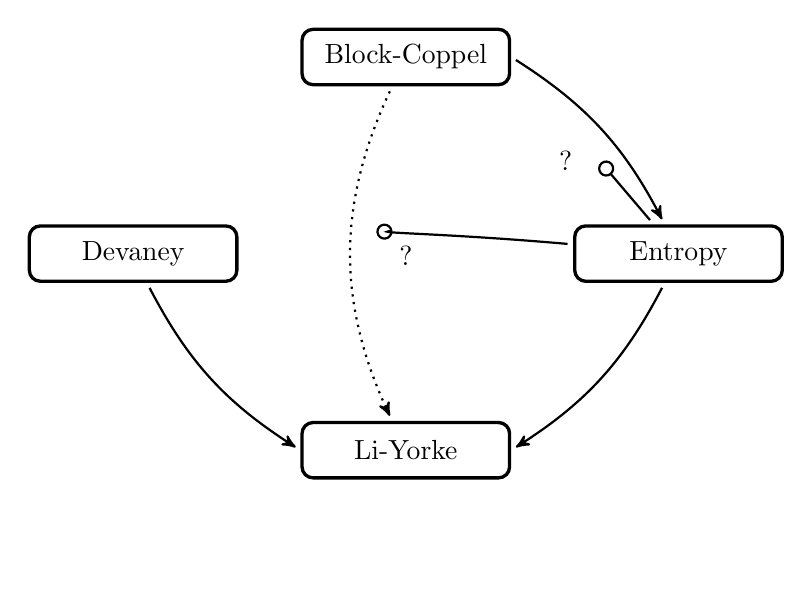
\begin{tikzpicture}[node distance=1cm, auto]
 %nodes
    \node[] (dummy) {};
    \node[box, inner sep=5pt,below=2.0cm of dummy] (ly) {Li-Yorke};
    \node[box, inner sep=5pt,left=2.0cm of dummy] (dev) {Devaney};
    \node[box, inner sep=5pt,above=2.0cm of dummy] (bc) {Block-Coppel};
    \node[box, inner sep=5pt,right=2.0cm of dummy] (entropy) {Entropy};
    \node[below=1.0cm of ly] (dummy2) {};
 %edges
    \draw[imply] (entropy)[bend left=15] to node {} (ly.east); 
    \draw[imply] (dev)[bend right=15] to node {} (ly.west); 
    \draw[imply] (bc.east) to [bend left=15] node {} (entropy); 
    \draw[induced] (bc)[bend right=25] to node {} (ly); 
    \draw[maybe] (entropy)[] to node {?} (bc.east); 
    \draw[maybe] (entropy)[bend right=5] to node {?} (dev); 
    %\draw[noinduced] (dev)[bend left=15] to node {} (bc.west); 
    %\draw[noimply] (ly)[] to node {} (entropy); 
    %\draw[noimply] (ly)[] to node {} (dev); 
    %\draw[noimply] (ly)[] to node {} (bc); 
    %\draw[noimply] (bc)[] to node {} (dev); 
    %\draw[noimply] (dev)[bend right=15] to node {} (entropy); 
  \end{tikzpicture}
  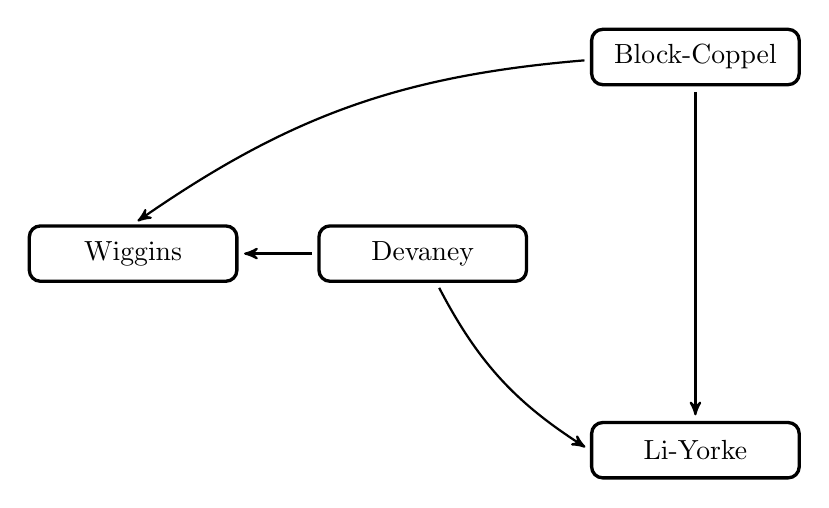
\begin{tikzpicture}[node distance=1cm, auto]
 %nodes
    \node[] (dummy) {};
    \node[box, inner sep=5pt,below=2.0cm of dummy] (ly) {Li-Yorke};
    \node[box, inner sep=5pt,left=2.0cm of dummy] (dev) {Devaney};
    \node[box, inner sep=5pt,left=1.0cm of dev] (wig) {Wiggins};
    \node[box, inner sep=5pt,above=2.0cm of dummy] (bc) {Block-Coppel};
 %edges
    \draw[imply] (dev)[bend right=15] to node {} (ly.west); 
    \draw[imply] (dev)[] to node {} (wig.east); 
    \draw[imply] (bc)[bend right=15] to node {} (wig.north); 
    \draw[imply] (bc)[] to node {} (ly); 
    %\draw[noinduced] (dev)[bend left=15] to node {} (bc.west); 
    %\draw[noimply] (ly)[] to node {} (entropy); 
    %\draw[noimply] (ly)[] to node {} (dev); 
    %\draw[noimply] (ly)[] to node {} (bc); 
    %\draw[noimply] (bc)[] to node {} (dev); 
    %\draw[noimply] (wig)[bend right=15] to node {} (ly); 
    %\draw[noimply] (dev)[bend right=15] to node {} (entropy); 
  \end{tikzpicture}
  \label{fig:chaos-metric}
  \caption{
    Relations between definitions for a compact metric space.
    An absence of an arrow means that the particular implication is not necessarily true.
    An arrow with a circular head (with a question mark) means it is an open question.
    An dotted arrow indicates a result that is not directly shown, but induced by other implications.
  }
\end{figure}
%%%


\subsubsection*{Topological Entropy and Li-Yorke}
As we have seen in the compact interval case that \liy does not imply $\pte$.
However, the converse still holds in this general setting.
\begin{theorem}
  If $(X,F)$ has positive topological entropy, then it is chaotic in Li-Yorke's sense.
  \label{thm:entropy-liyorke}
  \begin{proof}
    See \citet{blanchard}.
  \end{proof}
\end{theorem}
%%%

\subsubsection*{Block-Coppel and Topological Entropy}
\begin{theorem}
  If $(X,F)$ is chaotic in Block-Coppel's sense, then it has positive topological entropy.
  \begin{proof}
    $F$ is semi-conjugate to $\sigma: \Sigma \to \Sigma$, so that by Proposition~\ref{thm:ent-conj}, $h(\sigma) \leq h(F)$.
    Since $h(\sigma)$ is positive, we conclude that $h(F)$ is positive.
  \end{proof}
  \label{thm:blcp-entropy}
\end{theorem}
%
However, we do not know whether \pte implies \blcp.

%%%


\subsubsection*{Devaney and Topological Entropy}
\citet{glasner} provides an example of a symbolic system that is \dev but has zero entropy.
Hence, \dev does not imply \pte.
On the other hand, we do not know whether \pte implies \dev.
We have some related results, however.
\citet{glasner} proved that if a system is transitive, has no isolated point, and has positive topological entropy, then it is sensitive to initial conditions.
Thus, if we can prove that \pte implies the existence of a closed, invariant subset $Y \subseteq X$ on which $F$ is topologically transitive, then \pte implies \wig.
On the other hand, in order for \pte to imply \dev, \pte mush imply both \tt and \dpp.
While it seems plausible that topological transitivity follows from positive topological entropy, it seems unlikely that \pte implies the existence of dense periodic points.
%%%

\subsubsection*{Block-Coppel and Devaney/Wiggins}
\citet{aulbach} constructed an example to show that Block-Coppel's definition does not imply Devaney's definition.
\begin{example}
  \citep{aulbach} 
  Define $\tau: \Sigma \to \Sigma$ as the addition by $(1, 0, 0, \ldots) \in \Sigma$:
  \begin{equation*}
    \tau: s \mapsto s + (1, 0, 0, \ldots),
  \end{equation*}
  where the addition of two members of $\Sigma$ is defined in the same manner as the addition of two binary numbers.
  For example, 
  \begin{align*}
    (1, 0, 0, \ldots) + (1, 0, 0, \ldots) &= (0, 1, 0, \ldots) \\
    (0, 1, 0, \ldots) + (1, 0, 0, \ldots) &= (1, 1, 0, \ldots) \\
    (1, 1, 0, \ldots) + (1, 0, 0, \ldots) &= (0, 0, 1, \ldots).
  \end{align*}
  Also, we define $\tau(1,1,1, \ldots) \ceq (0,0,0, \ldots)$.
  It is easy to see that $\tau: \Sigma \to \Sigma$ is a homeomorphism, and does not have a periodic point of any period.
  Now, consider the dynamical system $(\Sigma \times \Sigma, F)$, where $F$ is defined as
  \begin{equation*}
    F: (s, t) \mapsto (\sigma(s), \tau(t)).
  \end{equation*}
  (Recall that $\sigma$ is the shift map.)
  $\Sigma$ is compact, so by Tychonoff's theorem, $\Sigma \times \Sigma$ is also compact.
  $(\Sigma \times \Sigma, F)$ is semi-conjugate to the one-sided full shift by $\pi_1$, the projection of the first component (i.e. $\pi_1 \circ F = \sigma \circ \pi_1$).
  Hence, the system is chaotic in Block-Coppel's sense.
  However, the system is not chaotic in Devaney's sense, because it doesn't have a periodic point.
  (Moreover, \citet{blockcoppel} proved that the system is also chaotic in Li-Yorke's sense.
  Therefore, \blcp together with \liy do not imply \dev.)
  $\square$
\end{example}
%%%
The system that we just introduced is not topologically transitive on $\Sigma \times \Sigma$.
However, it may still be possible to find a subset $Y$ of $\Sigma \times \Sigma$ such that $F_{|Y}$ is topologically transitive.
In fact, \citet{auslander} proved that it is possible to find such a subset.
In addition, \citet{auslander} showed that $F$ restricted to the subset is also sensitive to initial conditions; hence, \blcp implies \wig.

On the other hand, \dev does not imply \blcp.
We can deduce this from the results so far.
Suppose \dev implies \blcp.
Then \dev implies \pte; however, this is not necessarily the case, as shown before.
Therefore, \dev does not imply \blcp.

\subsubsection*{Block-Coppel and Li-Yorke}
\blcp implies \pte, and \pte implies \liy; these implications induces the implication from \blcp to \liy.
However, we know that the converse is not true from the compact interval case.
Hence, \blcp implies \liy, but the converse is not true.

\subsubsection*{Devaney/Wiggins and Li-Yorke}
The following example is a system that is chaotic in Wiggins's sense but not in Li-Yorke's sense.
\begin{example}
  \citep{blanchard}
  (Note to Rao: this example contains a few glitches, but I think the overall idea is right. I hope to discuss this at some point.)
  This example employs a \textit{two-sided shift}, a symbolic dynamical system on the set of all bi-infinite sequences.
  Since a two-sided shift is similar to an one-sided shift, instead of formally defining the dynamical system, we briefly discuss its structure here.
  Some of the results that we prove in this example are standard results for two-sided dynamical systems.
  Let $S = \set{0,1}$ be the set of symbols.
  In a two-sided shift system, $\Sigma \equiv S^\Z$ consists of bi-infinite sequences, i.e. sequences of the form
  \begin{align*}
    \cdots s_{-n} \cdots s_{-2} s_{-1} s_0 s_1 s_2 \cdots s_n \cdots.
  \end{align*}
  Also, we use the following metric on the space $\Sigma$ instead:
  \begin{equation*}
    \metric{a,b} = \frac{\delta_i}{2^{\abs{i}}},
  \end{equation*}
  where
  \begin{equation*}
    \delta_i = 
    \begin{cases}
      &0 \quad \mbox{ if } a_i = b_i  \\
      &1 \quad \mbox{ otherwise.}
    \end{cases}
\end{equation*}
  %This example uses a dynamical system commonly called the \textit{Sturmian system}.

  Let $S^1 \equiv [0, 1)$ be the unit circle, and let $R_\alpha: S^1 \to S^1$ be the rotation by an irrational number $\alpha \in S^1$. %]
  Recall that we showed in Chapter~\ref{chap:devaney} that the dynamical system $(S^1, R_\alpha)$ is topologically transitive, and has no periodic point.
  Note that $R_\alpha: S^1 \to S^1$ is one-to-one.
  For each point $x \in S^1$, $\phi: S^1 \to \Sigma$ sends $x$ to $s \in \Sigma$ such that
  \begin{equation*}
    s = \cdots s_{-n} \cdots s_{-1} s_0 s_1 \cdots s_n \cdots,
  \end{equation*}
  where
  \begin{equation*}
    s_i = \begin{cases}
      0& \mbox{ if } \itr{R_\alpha}{i}(x) \in [0, 1-\alpha)  \\
      1& \mbox{ if } \itr{R_\alpha}{i}(x) \in [1-\alpha, 1). %]
    \end{cases}
  \end{equation*}
  Let $X \ceq \phi(S^1)$.
  Then, since $\bar{X}$, the closure of $X$, is a closed subset of a compact space $\Sigma$, $\bar{X}$ is also compact.

  Also, $\bar{X}$ is invariant under the shift map $\sigma$.
  Suppose $s \in \bar{X}$.
  We may assume that there exists a sequence $\set{s_n} \subseteq X$ such that $\lim\limits_{n \to \infty} s_n = s$.
  For each $s_n$, there exists $\itr{\sigma}{-1}(s_n)$ that is a member of $\bar{X}$.
  Since $\sigma$ is homeomorphic, we have $\lim\limits_{n \to \infty} \itr{\sigma}{-1}(s_n) = \itr{\sigma}{-1}(s)$.
  It follows that $s \in \sigma(\bar{X})$; hence, $\bar{X} \subseteq \sigma(\bar{X})$.
  A similar argument shows that $\sigma(\bar{X}) \subseteq \bar{X}$.
  Hence, $\sigma(\bar{X}) = \bar{X}$.
  (The reason that we proved that $\bar{X}$ is a compact, invariant subset of $\Sigma$ is not only because Wiggins's definition calls for the conditions to be satisfied on a compact set.
  As it turns out, these conditions are required for a symbolic dynamics to be well-defined.
  See \citep[p.179]{lind}.)
  
  Next, we show that $\phi$ is a continuous mapping.
  Fix $\epsilon > 0$.
  We may assume that $2^{-k} < \epsilon$.
  By Proposition~\ref{prop:two-sided}, which we prove immediately after this example, for any $k$, $\phi(x)_i = \phi(y)_i$ for $0 \leq \abs{i} \leq k+1$ implies that
  \begin{equation*}
    \metric{\phi(x),\phi(y)} \leq 2^{-k}.
  \end{equation*}
  Therefore, we only need to prove that, for each $x \in S^1$, there exists $y \in S^1$ such that $x_i = y_i$ for $0 \leq \abs{i} \leq k+1$.
  It is easy to see that $\phi(x)_i \neq \phi(y)_i$ if and only if $0 \in (\phi(x)_i, \phi(y)_i]$ or $1 - \alpha \in (\phi(x)_i, \phi(y)_i]$. %)
  So for each $x$, let $y = x + \delta$ for some $\delta > 0$.
  If 
  \begin{equation*}
    0 \in R_\alpha((x, x+\delta]) \mbox{ or } 1 - \alpha \in R_\alpha((x, x+\delta]), 
  \end{equation*}
   then we can redefine $\delta$ to be a smaller value so that 
   \begin{equation*}
     0, 1-\alpha \not\in R_\alpha((x, x+\delta]). %)))
   \end{equation*}
  Inductively, we see that, for any $k \in \N$, if $\delta$ is small enough, then 
  \begin{equation*}
    0, 1-\alpha \not\in \itr{R_\alpha}{k+1}(x, x+\delta) 
  \end{equation*}
  so that
  \begin{equation*}
    \phi(x)_i = \phi(x+\delta)_i \mbox{ for } 0 \leq \abs{i} \leq k+1.
  \end{equation*}
  Thus, $\phi$ is continuous.
  (Incorrect.. $\phi$ isn't continuous at $0, 1-\alpha \in S^1$. Need to do something about it.
  One idea is to cover $S^1$ with $[0,1-\alpha]$ and $[1-\alpha, 1]$.
  )

  Now, we prove that $(\sigma, \bar{X})$ is chaotic in Wiggins's sense.
  The fact that $R_\alpha: X \to X$ is topologically transitive implies that $R_\alpha: \bar{X} \to \bar{X}$ is also topologically transitive (See Proposition~\ref{prop:closure-transitivity}).
  For the system to be chaotic in Wiggins's sense, $\sigma$ needs to be sensitive to initial conditions on $\bar{X}$.
  Let $0 < \delta < 1$ be our separation constant.
  For any given $x \in S^1$, and $\epsilon > 0$, we can find $y \in \oball{\epsilon}{x}$ by the argument we gave in proving the continuity of $\phi$.
  Without loss of generality, we may assume that $y > x$.
  Then, let $z$ be the midpoint of the interval $(x,y)$, and $\eta \ceq \frac{\metric{x,y}}{2}$, so that $(z-\eta, z+\eta) = (x,y)$.
  Since $R_\alpha$ is transitive, there exists $m \geq 0$ such that 
  \begin{equation*}
    \itr{R_\alpha}{m}(z) \in \oball{\eta/2}{0}.
  \end{equation*}
  $R_\alpha$ is an isometry, so
  \begin{equation*}
    \oball{\eta/2}{0} \subseteq \itr{R_\alpha}{m}(z-\eta, z+\eta) 
    = \itr{R_\alpha}{m}(x,y).
  \end{equation*}
  Hence, $0 \in \itr{R_\alpha}{m}(x,y)$.
  It follows that $\phi(x)_m \neq \phi(y)_m$.
  Therefore,
  \begin{equation*}
    \metric{\itr{\sigma}{m}(x), \itr{\sigma}{m}(y)} \geq 1 > \delta.
  \end{equation*}
  Thus, $(\sigma, \bar{X})$ is chaotic in Wiggins's sense.
  
  By the same argument in proving \sdic, we see that, for each $x,y \in \bar{X}$, there are infinitely many $n$ such that 
  \begin{equation*}
    \metric{\itr{\sigma}{n}(x),\itr{\sigma}{n}(y)} > 0.
  \end{equation*}
  Hence, $\liminf\limits_{n \to \infty} (\itr{\sigma}{n}(x), \itr{\sigma}{n}(x+\delta)) > 0$, so that $(\sigma, \bar{X})$ is not chaotic in Li-Yorke's sense.
  $\square$
\end{example}
\begin{proposition}
  Let $x,y$ be members of $\Sigma$.
  If $x_i = y_i$ for $0 \leq \abs{i} \leq k$, then $\metric{x,y} \leq 2^{-(k-1)}$.
  \label{prop:two-sided}
  \begin{proof}
    $\metric{x,y}$ achieves its upper bound when $x_i \neq y_i$ for $\abs{i} \geq k+1$.
    \begin{align*}
      \metric{x,y}
      &\leq 2 \cdot \sum\limits_{n = k+1}^{\infty} \frac{1}{2^{\abs{i}}} \\
      &\leq 2 \cdot \paren{ \sum\limits_{n = 0}^{\infty} \frac{1}{2^{\abs{i}}} - \sum\limits_{n = 0}^{k} \frac{1}{2^{\abs{i}}}} \\
      &= 2 \cdot (2 - (2 - \frac{1}{2^k})) \\
      &= \frac{1}{2^{k-1}}.
    \end{align*}
  \end{proof}
\end{proposition}
\begin{proposition}
  Let $F: X \to X$ be a continuous map, $Y$ be a subset of $X$.
  If $F$ restricted to $Y$ is topologically transitive, then $F: \bar{Y} \to \bar{Y}$ is also transitive.
  \label{prop:closure-transitivity}
  \begin{proof}
    Since $F$ is transitive on $Y$, for each $U, V \subseteq Y$, there exists $n$ such that
    \begin{equation*}
      \itr{F}{n}(\interior(\bar{U})) \cap \interior(\bar{V}) \neq \emptyset.
    \end{equation*}
    It follows that
    \begin{equation*}
      \itr{F}{n}(\bar{U}) \cap \bar{V} \neq \emptyset.
    \end{equation*}
  \end{proof}
\end{proposition}

%%%
\begin{theorem}
  If $(X, F)$ is chaotic in Devaney's sense, then it is chaotic in Li-Yorke's sense.
  \begin{proof}
    See \citet{mai}.
    \citet{huang} also proved the same result.
  \end{proof}
  \label{thm:dev-liy}
\end{theorem}
More specifically, Mai proved that, for a complete metric space $X$ without an isolated point, if $F: X \to X$ is transitive and has a periodic point of any period, then $F$ is chaotic in Li-Yorke's sense.
Thus, even though \tt and \sdic do not imply Li-Yorke's chaos, as we saw in the Sturmian system, \tt and the existence of a \textit{single} periodic point, which is significantly weaker than \dpp, imply chaos in Li-Yorke's sense.
This result may be instructive in evaluating whether \dpp in Devaney's definition is too strong.
Also, we can make an interesting observation from the fact that \wig and \liy do not imply each other. 
Recall that, though it is not explicitly called sensitivity, Li-Yorke's definition uses its own version of sensitivity, $\limsup\limits_{n\to \infty} \metric{\itr{F}{n}(x), \itr{F}{n}(y)} > 0$, called the \textit{non-asymptotic relation}.
The non-asymptotic relation is analogous to, yet different from \sdic used in Devaney's and Wiggins's definitions.
In the same manner, we can see that the other condition, the \textit{proximal relation}, in Li-Yorke's definition, $\liminf\limits_{n\to \infty} \metric{\itr{F}{n}(x), \itr{F}{n}(y)} = 0$, is similar to topological transitivity.
The result about \wig and \liy indicates that non-asymptotic and proximal relations are neither stonger nor weaker than \tt and \sdic, even though these conditions contain similar ideas.
%%%

\subsubsection*{Result}
As in the compact interval case, each of \dev, \blcp, and \pte implies \liy.
However, the three definition that are equivalent for a compact inteval are no longer equivalent in a general compact metric space (Figure~\ref{fig:chaos-metric}).
Also, there are open questions.
We do not know whether \pte implies \blcp or \dev.
We obtain the implication from \pte to \wig if \pte implies the existence of a subset $Y$ such that $F_{|Y}$ is topological transitive.
We may also be interested in looking at individual conditions in each definition.
For example, we may ask: does topological transitivity imply positive topological entropy?

We have a few more things to say about Devaney's definition now.
We saw that a single periodic point in addition to \wig is a sufficient condition to imply \liy. 
This result suggests that requiring the existence of dense periodic points may be too restrictive.
As we mentioned in Chapter~\ref{chap:devaney}, \citet{glasner} proposed that requiring a dense set of periodic points is too restrictive, and suggested alternative conditions, one of which is the existence of an invariant measure that is positive on each non-empty open set.
Also, the contrast of \dev and \wig seen through their relations with \pte and \liy (Figure~\ref{fig:chaos-metric}; the second diagram) is noteworthy.
\dev implies \liy, but \wig does not.
This is because \wig is weaker than \dev, and by the same reason, \blcp implies \wig, but not \dev.

\bibliographystyle{../../bibliography/pjgsm}
\bibliography{../../bibliography/thesis}

\printindex

%\section{Conclusion}
%Work in progress
%We have concentrated on the comparisons of definitions, but the field of dynamical systems is more than just that.
%For example, one may be interested in finding what conditions imply \sdic.
%We proved that \dpp and \tt are sufficient conditions for \sdic, but can we use a weaker condition to derive \sdic?
%Are there other conditions that imply \sdic?
%Do topologically transitive maps have positive topological entropy?
%One could define chaos for measure-theoretic dynamics \citep{downarowicz} or differentiable dynamical systems \citep{ruellebook}.
%One could also study how complicated dynamics arise.
%For example, period doubling route to chaos and intermittency route to chaos \citep{sternbergbook}
%
%\subsection*{Some Open Problems}
%\begin{enumerate}
%  \item Steve's problem
%  \item Does topological transitivity imply positive topological entropy?
%\end{enumerate}


\end{document}
